\documentclass{beamer}
\usepackage[latin1]{inputenc}
\usepackage{graphics}
\usepackage{listings}
\usepackage{graphicx}
\usetheme{Warsaw}
\title[Using Git like a baus]{Crash course in revision control\\Or how to be a good employee}
\author{Phillip Whittlesea - DevECS}
\institute{Electronics and Computer Science}

\lstset{
language=bash,
basicstyle=\footnotesize
}
\newcommand{\demo}[1]{\begin{exampleblock}{To the command line!}#1\end{exampleblock}}
\newcommand{\clfact}[2]{\begin{alertblock}{In short...}\textbf{#1} #2\end{alertblock}}
\begin{document}

\begin{frame}
    \titlepage
\end{frame}

\begin{frame}{Introduction}
    What we are going to cover today:
    \begin{enumerate}
        \item Why do we all use revision control?
        \item What is revision control?
        \item Git
    \end{enumerate}
\end{frame}

\begin{frame}{Who here has lost work?}
\huge \centering
Who here has never lost work?
\end{frame}

\begin{frame}{Why do we use revision control?}
    \begin{figure}[ht]
        \centering
        
\includegraphics[width=0.8\linewidth]{img/losing.jpg}
        \caption{Not using revision control is always a bad choice}
        \label{fig:figure2}
    \end{figure}
\end{frame}

\begin{frame}{Why do we use revision control?}
    \begin{figure}[ht]
        \centering
        
\includegraphics[width=0.8\linewidth]{img/winning.jpg}
        \caption{This is what happens when you use Revision Control}
        \label{fig:figure1}
    \end{figure}
\end{frame}

\begin{frame}{The number one rule for revision control?}
\centering
\huge
Use It! 
\end{frame}

\begin{frame}{What is revision control?}
    \begin{itemize}
        \item More commonly known as "Source Control Management" (SCM)
        \pause
        \item Two major types:
        \begin{itemize}
            \item Centralised SCM
            \begin{itemize}
                \item Server: The Repository
                \item Client: Local changes
            \end{itemize}
            \pause
            \item Decentralised SCM
            \begin{itemize}
                \item Anyone can be the server %(GDP)
                \item Complete history
                \item Offline usage
            \end{itemize}
        \end{itemize}  
    \end{itemize}  
\end{frame}

\begin{frame}{Git: A Decentralised SCM}
    \begin{block}{Just remember, you have everything locally}
    \begin{figure}[ht]
        \centering
        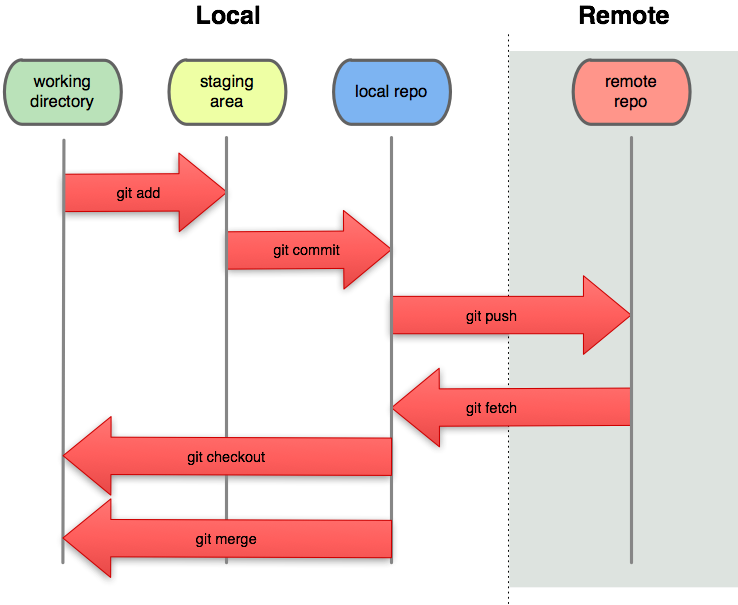
\includegraphics[width=0.6\linewidth]{img/overview.png}
        \caption{Git has several layers allowing for complete control\footnote{Image from \href{http://whygitisbetterthanx.com/}{http://whygitisbetterthanx.com/}}}
        \label{fig:figure0}
    \end{figure}
    \end{block}
\end{frame}

\begin{frame}{Under the hood?}
    \begin{block}{Google it!}
        It can get pretty advanced pretty quickly
    \end{block}
\end{frame}

\begin{frame}{Time to rock and roll}
    \begin{block}{Lets get it started...}
        Time for you guys to join in!
        Steps to follow:
        \begin{enumerate}
            \item Have a computer with git OR ssh into linuxproj
            \item Have a GitHub account
        \end{enumerate}
    \end{block}
\end{frame}
\begin{frame}{To GitHub!}
    \begin{exampleblock}{Creating a repository}
        Lets start simple and start a project on GitHub
    \end{exampleblock}
\end{frame}

\begin{frame}{Git init}
    \begin{block}{Git init, or, where do baby repositories come from}
    \textbf{In a nutshell}, you use git init to make an existing directory of content into a new Git repository.
    You can do this in any directory at any time, completely locally.
    \lstinputlisting{code/gitinit.sh}
    \end{block}
    \clfact{git init}{initializes a directory as a Git repository}
\end{frame}
\demo{Creating our repository}

\begin{frame}{Git status}
    \begin{block}{Git status, or, 'Hey Git whats happening?'}
    \textbf{In a nutshell}, you run git status to see if anything has been modified since your last commit so you can decide if you want to commit.
    \lstinputlisting{code/gitstatus.sh}
    \end{block}
    \clfact{git status}{view the status of your files in the working directory}
\end{frame}
\demo{Finding out what Git knows}

\begin{frame}{Git add}
    \begin{block}{Git add, or, what to do if you like your changes}
    \textbf{In a nutshell}, you run git add on a file when you want to include whatever changes you've made to it in your next commit.
    \lstinputlisting{code/gitadd.sh}
    \end{block}
    \clfact{git add}{adds file contents to the staging area}
\end{frame}
\demo{Telling Git what to remember}

\begin{frame}{The Staging Area}
    \begin{block}{Stop the press, what is a staging area?!}
    \textbf{In a nutshell}, think of the staging area as a loading dock before your truckload of code heads off to Commitsville\footnote{Image from \href{http://whygitisbetterthanx.com/}{http://whygitisbetterthanx.com/}}.
    \begin{figure}[ht]
        \centering
        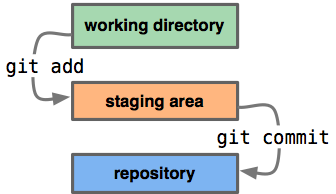
\includegraphics[width=0.5\linewidth]{img/staging.png}
        \label{fig:figure3}
    \end{figure}
    \end{block}
\end{frame}

\begin{frame}{Git commit}
    \begin{block}{Git commit, or, lets keep that as its kinda important}
    \textbf{In a nutshell}, you run git commit to record the snapshot of your staged content. This snapshot can then be compared, shared and reverted to if you need to.
    \lstinputlisting{code/gitcommit.sh}
    \end{block}
    \clfact{git commit}{records a snapshot of the staging area}
\end{frame}
\demo{Telling Git that you REALLY want this}

\begin{frame}{Git remote}
    \begin{block}{Git remote, or, where did I leave that repository?}
    \textbf{In a nutshell}, with git remote you can list remote repositories. Use git remote add to add new remotes and git remote rm to delete existing ones.
    \lstinputlisting{code/gitremote.sh}
    \end{block}
\end{frame}

\begin{frame}{Git push}
    \begin{block}{Git push, or, sharing is caring!}
    \textbf{In a nutshell}, you run git push to update a remote repository with the changes you've made locally. 
    \lstinputlisting{code/gitpush.sh}
    \end{block}
    \pause
    \demo{Deploying local code to a remote location}
\end{frame}

\begin{frame}{Git pull / fetch + merge; bring it back now y'all!}
    \begin{block}{Git fetch + merge}
    \textbf{Git fetch}, will pull changes from the remote to the local repo.

    \textbf{Git merge}, will merge a branch into the current context. 
    \end{block}
\centering \textbf{OR}
    \begin{block}{Git pull}
    \textbf{In a nutshell}, you run git pull to take the latest changes from the remote repository. 
    \end{block}
\end{frame}

\begin{frame}{tldr; What we've covered...}
    \begin{figure}[ht]
        \centering
        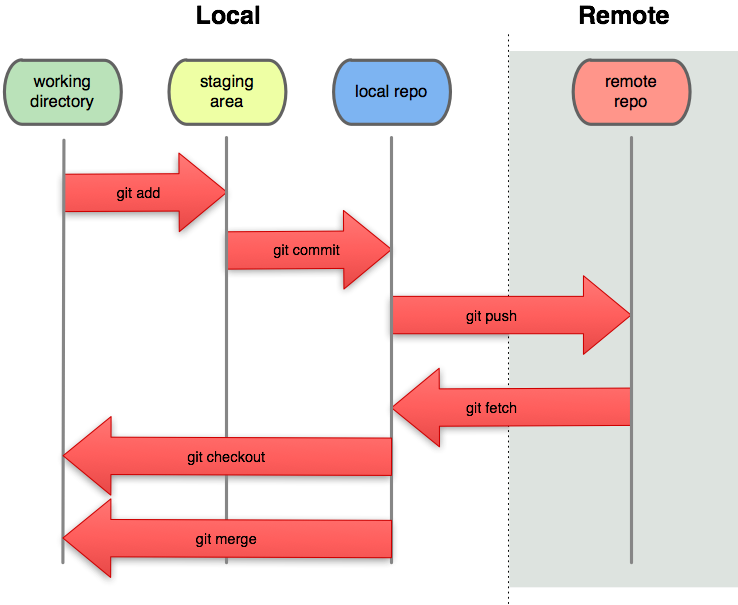
\includegraphics[width=0.8\linewidth]{img/overview.png}
        \caption{Don't forget git pull!}
        \label{fig:figure10}
    \end{figure}
\end{frame}
%\begin{frame}{Bring on the trumpets!}
%    \begin{block}{Thats all folks!}
%        So where do we go from here?
%        \begin{enumerate}
%            \item \textbf{Leave} if, like Jason Derulo, you're ridin' solo!
%            \item \textbf{Stay} and we'll go more pro with Git!
%        \end{enumerate}
%    \end{block}
%    \begin{figure}[ht]
%        \centering
%        
\includegraphics[width=0.8\linewidth]{img/pleasestay.png}
%    \end{figure}
%\end{frame}

%\begin{frame}{Git Diff}
    \begin{block}{Git Diff: a Goldfishes best friend}
    \textbf{In a nutshell}, you run git diff to see how files have been modified or staged on a line by line basis.
    \lstinputlisting{code/gitdiff.sh}
    \end{block}
    \clfact{git commit}{shows diff of what is staged and what is modified but unstaged}
\end{frame}
\demo{Finding out what we did before your Mum rang}

\begin{frame}{Git Branch}
    \begin{block}{Git Branch, or, programming your bit on the side!}
    \textbf{In a nutshell}, you use git branch to list your current branches, create new branches and delete unnecessary or already merged branches. 
    \begin{figure}[ht]
        \centering
        
\includegraphics[width=0.40\linewidth]{img/branching.png}
        \caption{A single git repository can maintain multiple branches of development.}
    \end{figure}
    \end{block}
    \pause
    \demo{Creating a branch for some simple changes}
\end{frame}

\begin{frame}{Other matters...}
    git tag
    git log
    Who needs folders? Git wont create empty folders
\end{frame}

\end{document}
